\documentclass[a4paper, 10.5pt, twocolumn, dvipdfmx]{jarticle}

\usepackage{natbib} % 文献参照作成
\usepackage[dvipdfmx,setpagesize=false]{hyperref} % ハイパーリンク対応
\usepackage{amsmath,amssymb} % 数式作成
\usepackage{array} % 数式作成
\usepackage{booktabs} % 表に横罫線を引く
\usepackage{multirow} % 表中でセル結合する
\usepackage{bigdelim} % 行列に括弧を付与する
\usepackage{fancybox} % 文章を枠や円で囲む
\usepackage{makeidx} % 索引作成
\usepackage{comment} % 複数行のコメントアウト
\usepackage[dvipdfmx]{graphicx} % 画像読み込み
\usepackage{float} % 図表の位置を操作する
\usepackage{lscape} % 図表を90°回転させる
\usepackage{tabularx} % 表の幅を調整する
\usepackage{scalefnt} % 文字を拡大縮小する
\usepackage{bm} % 文字を太字にする
\usepackage{etoolbox} % コマンドをカスタマイズする
 % パッケージ読み込み
\makeatletter % "@"記号の有効化

\makeindex
\setcounter{tocdepth}{2}

%%% セクション構成の設定 %%%
\renewcommand{\section}{%
	\@startsection {section}{1}{\z@}% セクション表記の設定
	{-2.5ex plus -1ex minus -.2ex} % 前の行間を縮める
	{1.5ex plus .2ex} % 後の行間を縮める
	{\sf\bf}% セクションのフォント設定
}

\renewcommand{\subsection}{% サブセクション表記の設定
	\@startsection {subsection}{1}{\z@}%
	{-2.5ex plus -1ex minus -.2ex} % 前の行間を縮める
	{1.5ex plus .2ex}% 後の行間を縮める
	{\bf}% サブセクションのフォント設定
}


%%% ページレイアウトの設定 %%%
\setlength{\topmargin}{-7.4truemm} % 上の余白
\setlength{\oddsidemargin}{25mm} % 左の余白
\iftombow % トンボがある場合
	\addtolength{\oddsidemargin}{-1in} % トンボの分だけ左にずらす
\else
	\addtolength{\oddsidemargin}{-1truein} % トンボの分だけ左にずらす
\fi
\setlength{\headheight}{1mm} % ヘッダの高さ
\setlength{\headsep}{1mm} % ヘッダと本文の間隔
\setlength{\textwidth}{48zw} % 1行48文字(二段組の場合は24文字)
\setlength{\textheight}{46\baselineskip} % 1ページ42行程度(適宜微調整して下さい)
\addtolength{\textheight}{\topskip} % 本文とフッタの間隔
% \setlength{\parindent}{1em} % 段落のインデントを1文字分に設定


%%% ヘッダー・フッターの設定 %%%
\pagestyle{fancy}
\fancyhf{} % すべてのヘッダーとフッターをクリア
\renewcommand{\headrulewidth}{0.0pt} % ヘッダーの下の線を消す
\renewcommand{\footrulewidth}{0.0pt} % フッターの上の線を消す
% 1ページ目のスタイルを設定
\fancypagestyle{firstpage}{
	\fancyhf{} % すべてのヘッダーとフッターをクリア
	\renewcommand{\headrulewidth}{0.0pt} % ヘッダーの下の線を消す
	\renewcommand{\footrulewidth}{0.8pt} % フッターの上の線を太くする
	\fancyfoot[L]{{\small キーワード:社会資本投資,地域経済,計量経済モデル,GDP成長,所得分配}} % フッターの左側にキーワードを表示
}
% 2ページ目以降のスタイルを設定
\fancypagestyle{plain}{
	\fancyhf{} % すべてのヘッダーとフッターをクリア
	\renewcommand{\headrulewidth}{0.0pt} % ヘッダーの下の線を消す
	\renewcommand{\footrulewidth}{0.0pt} % フッターの上の線を消す
}


%%% 引用スタイルの設定 %%%
\renewcommand{\bibname}{参考文献} % 参考文献のタイトル
\setcitestyle{super,sort&compress,citesep={,},open={},close={)}}  % 参考文献の引用形式(natbib)
\setlength{\bibsep}{0pt} % 参考文献リストの行間を狭くする
% \renewcommand{\bibsection}{\chapter*{\bibname}}

%%% 参考文献リストの行間をさらに狭くする設定 %%%
\renewenvironment{thebibliography}[1]
{\section*{\refname\@mkboth{\refname}{\refname}}%
	\list{\@biblabel{\@arabic\c@enumiv}}%
	{\settowidth\labelwidth{\@biblabel{#1}}%
		\leftmargin0pt % インデントをゼロにする
		\advance\leftmargin\labelsep
		\setlength\itemsep{0pt} % 行間を狭くする
		\setlength\parsep{0pt} % 行間を狭くする
		\setlength\baselineskip{9pt} % 文字の大きさを調整
		\setlength{\labelsep}{0.5em} % ラベルと本文の間のスペースを調整
		\setlength{\labelwidth}{1em} % ラベルの幅を調整
		\@openbib@code
		\usecounter{enumiv}%
		\let\p@enumiv\@empty
		\renewcommand\theenumiv{\@arabic\c@enumiv}}%
	\sloppy
	\clubpenalty4000
	\@clubpenalty\clubpenalty
	\widowpenalty4000%
	\sfcode`\.\@m
	\setlength{\parindent}{0pt} % 参考文献リスト内のインデントを無効にする
}
{\def\@noitemerr
	{\@latex@warning{Empty `thebibliography' environment}}%
	\endlist}


%%% 数式の文字サイズを小さく設定 %%%
\everydisplay{\small} % ディスプレイ数式の文字サイズを小さくする

%%% 数式の文字間隔を狭く設定 %%%
\setlength{\thinmuskip}{0.5mu} % 通常の数式の間隔を狭くする
\setlength{\medmuskip}{1mu}  % 中程度の数式の間隔を狭くする
\setlength{\thickmuskip}{1mu} % 太い数式の間隔を狭くする


%%% その他の設定 %%%
\renewcommand{\baselinestretch}{1} % 行間の大きさ(倍率)
\setcounter{tocdepth}{2} % 目次のセクションの深さ(章(chapter), 節(section), 小節(subsection)の0~2段階)
\setcounter{MaxMatrixCols}{20} % 行列の最大列数
\pgfplotsset{compat=1.18}



\makeatother % "@"記号の有効化をオフ
   % ドキュメント設定
\makeatletter % "@"記号の有効化

\newcommand{\ES}{\begin{align}} % \begin{align}の簡略化
\newcommand{\EF}{\end{align}} % \end{align}の簡略化
\newcommand{\figcaption}[1]{\def\@captype{figure}\caption{#1}} % 図のキャプション機能
\newcommand{\tblcaption}[1]{\def\@captype{table}\caption{#1}} % 表のキャプション機能
\newcommand{\eqnum}{\addtocounter{align}{1}\tag*{\normalsize{(\arabic{align})}}} % 数式番号の付与機能(align環境)
\newcommand{\BigFig}[1]{\parbox{12pt}{\Huge #1}} % 強調文字の機能

\newcommand{\kintou}[2]{ % 文字の均等割付けの機能
  \leavevmode
  \hbox to #1{%
    \kanjiskip=0pt plus 1fill minus 1fill
    \xkanjiskip=\kanjiskip
    #2}%
}
\setcounter{tocdepth}{2}

\newcommand{\ctext}[1]{ % 丸囲み文字(①など)の機能
  \raise0.2ex\hbox{\textcircled{\scriptsize{#1}}}%
}

\makeatother % "@"記号の有効化をオフ
   % マクロ定義

\begin{document}
\thispagestyle{firstpage}

\twocolumn[
	\begin{center}
		{\large {\bf 社会資本投資が地域経済に与える影響の実証分析}}%タイトル
	\end{center}

	\begin{flushright}
		\kintou{6zw}{市民工学専攻}:神戸 太郎\\
		\kintou{6zw}{指導教員}: 灘 和美
	\end{flushright}
]


\section{はじめに}
社会資本投資は,インフラ整備を通じて地域経済の活性化や住民の生活の質向上に寄与する重要な政策手段である.しかし,その具体的な効果については,地域特性や投資対象の種類,投資規模によって異なり,明確な結論に至っていない部分も多いのが現状である.特に,地方都市や過疎地域では,社会資本投資がどの程度地域経済に波及効果をもたらすのか,また,その効果が持続可能な形で現れるのかを定量的に示す必要がある.

本研究の目的は,社会資本投資が地域経済に及ぼす影響を実証的に明らかにし,その波及効果を定量的に評価することである.具体的には,社会資本投資が地域の雇用創出や所得向上,生産性向上にどのような形で寄与するかを検証し,政策効果を科学的に測定することを目指す.

特に,地域特性や経済的条件の違いが投資効果に与える影響を詳細に分析することで,投資の効率性を高める方策を提案する.また,短期的な経済効果だけでなく,長期的な持続可能性や地域間格差への影響についても検討を行い,政策立案に資する実践的な知見を提供する.

\section{既往研究の整理と本研究の位置付け}
社会資本投資が地域経済に与える影響について,多くの実証研究が行われている.御園(2014)\cite{misono2014}は,日本の社会資本が地域別生産性に与える効果を再検証し,社会資本ストックが生産性向上に寄与することを示した.また,金(2013)\cite{kim2013}は,社会資本や公共投資の経済効果に関する実証研究を行い,公共投資が短期的な需要面への効果を持つことを指摘している. これらの研究は,社会資本投資が地域経済に与える影響を理解する上で重要な知見を提供しているが,地域特性や投資の種類,規模によって効果が異なるため,さらなる分析が求められる.


本研究は,地域間の付加価値成長率と全要素生産性(TFP)を従属変数とし,社会資本投資が地域経済に与える影響を実証的に分析することを目的とする.特に,社会資本投資の経済効果を地域特性や投資規模の観点から評価し,その効果の異質性や波及メカニズムを明らかにすることに新規性を持つ.また,マクロ経済モデルを活用し,短期的な効果にとどまらず,長期的な持続可能性や地域間格差の是正に対する社会資本投資の役割を解明することを目指す.

さらに,本研究は,公共投資の効率性を向上させるための基盤的な知見を提供することを意図している.具体的には,社会資本投資がどのようにして地域の経済成長や生産性向上を支えるのかを詳細に分析し,効率的な資源配分や政策立案に資する実践的な指針を提示する.本研究の成果は,学術的な貢献に加え,地域経済政策における社会資本投資の最適なあり方を探る上での新たな示唆を与えるものである.


\section{モデルの定義}
本研究では,社会資本投資が地域経済に与える影響を実証的に分析するため,地域間の付加価値成長率および全要素生産性(TFP)を従属変数とした回帰分析を行う.独立変数としては,社会資本投資額や社会資本ストック指標を中心に,各地域の経済特性を反映する補足変数(人口密度,産業構造,教育水準など)を組み込むことで,投資効果の多面的な評価を可能にする.


地域 \( i \) における生産量 \( Y_i \) は次のように定義する:

\[
	Y_i = A_i \cdot K_i^\alpha \cdot L_i^\beta \cdot G_i^\gamma
\]

ここで:
\begin{itemize}
	\renewcommand{\labelitemi}{}
	\item \( Y_i \) は地域 \( i \) の生産量(付加価値など)
	\item \( A_i \) は全要素生産性(TFP)
	\item \( K_i \) は民間資本ストック
	\item \( L_i \) は労働投入量
	\item \( G_i \) は社会資本ストック
	\item \( \alpha, \beta, \gamma \) は資本,労働,社会資本の生産弾力性(\( \alpha + \beta + \gamma \leq 1 \))
\end{itemize}

\subsection{社会資本ストックの動学的変化}

社会資本ストック \( G_i \) は,時間 \( t \) における社会資本投資 \( I_{G,i}(t) \) によって次のように変化する:

\[
	G_i(t+1) = (1-\delta) \cdot G_i(t) + I_{G,i}(t)
\]

ここで:
\begin{itemize}
	\renewcommand{\labelitemi}{}
	\item \( \delta \) は社会資本の減耗率(\( 0 < \delta < 1 \))
	\item \( I_{G,i}(t) \) は時点 \( t \) における社会資本投資
\end{itemize}

\subsection{TFPへの波及効果}

全要素生産性 \( A_i \) は,以下のように社会資本ストックの外部効果を含む:

\[
	A_i = A_0 \cdot e^{\phi \cdot G_i}
\]

ここで:
\begin{itemize}
	\renewcommand{\labelitemi}{}
	\item \( A_0 \) は基本的なTFP水準
	\item \( \phi \) は社会資本ストックがTFPに与える効果の強度
\end{itemize}

社会資本投資に関するデータは,国土交通省が提供する社会資本ストック統計および社会資本投資額の統計を利用し,地域ごとの社会資本整備の状況を把握する.地域経済の付加価値成長率や全要素生産性(TFP)の計算には,内閣府が提供する地域別経済統計を活用する.加えて,人口密度や産業構造,教育水準といった地域特性を表すデータは,総務省の「国勢調査」や「経済センサス」から取得する.

\section{結果と考察}
本研究では,社会資本投資が地域経済に与える影響を分析するため,回帰モデルを適用した実証分析を行った.従属変数として経済成長率を用い,独立変数として社会資本投資額,民間資本,労働投入量を組み込み,回帰分析を実施した.

表 \ref{tab:regression_results} に回帰分析の結果を示す.社会資本投資の係数は \( 0.0546 \)(\( p < 0.01 \))であり,他の条件が一定の場合,社会資本投資額の増加が経済成長率を増加させることが示された.また,民間資本と労働投入量も統計的に有意な正の影響を与えることが分かった.

さらに,社会資本投資と経済成長率の関係を視覚的に示すため,図 \ref{fig:regression_plot} に回帰直線を描画した.観測データと回帰直線の比較により,社会資本投資額が増加するほど経済成長率が高まる傾向が明確に観察された.この結果は,社会資本投資が直接的な生産要素としてだけでなく,間接的な経済波及効果をもたらす可能性を支持するものである.

\begin{table}[h!]
  \centering
  \renewcommand{\arraystretch}{1.2}
  \begin{tabular}{lrr}
  \toprule
  \textbf{変数}                    & \textbf{係数} & \textbf{P値} \\
  \midrule
  定数項 (Intercept)              & -0.598        & 0.212 \\
  社会資本投資 (Social Capital)    & 0.0546        & $<0.01$ \\
  民間資本 (Private Capital)       & 0.0314        & $<0.01$ \\
  労働投入量 (Labor)               & 0.0108        & $<0.01$ \\
  \bottomrule
  \end{tabular}
  \caption{回帰分析の結果}
  \label{tab:regression_results}
  \end{table}
  

\begin{figure}[!ht]
	\centering
	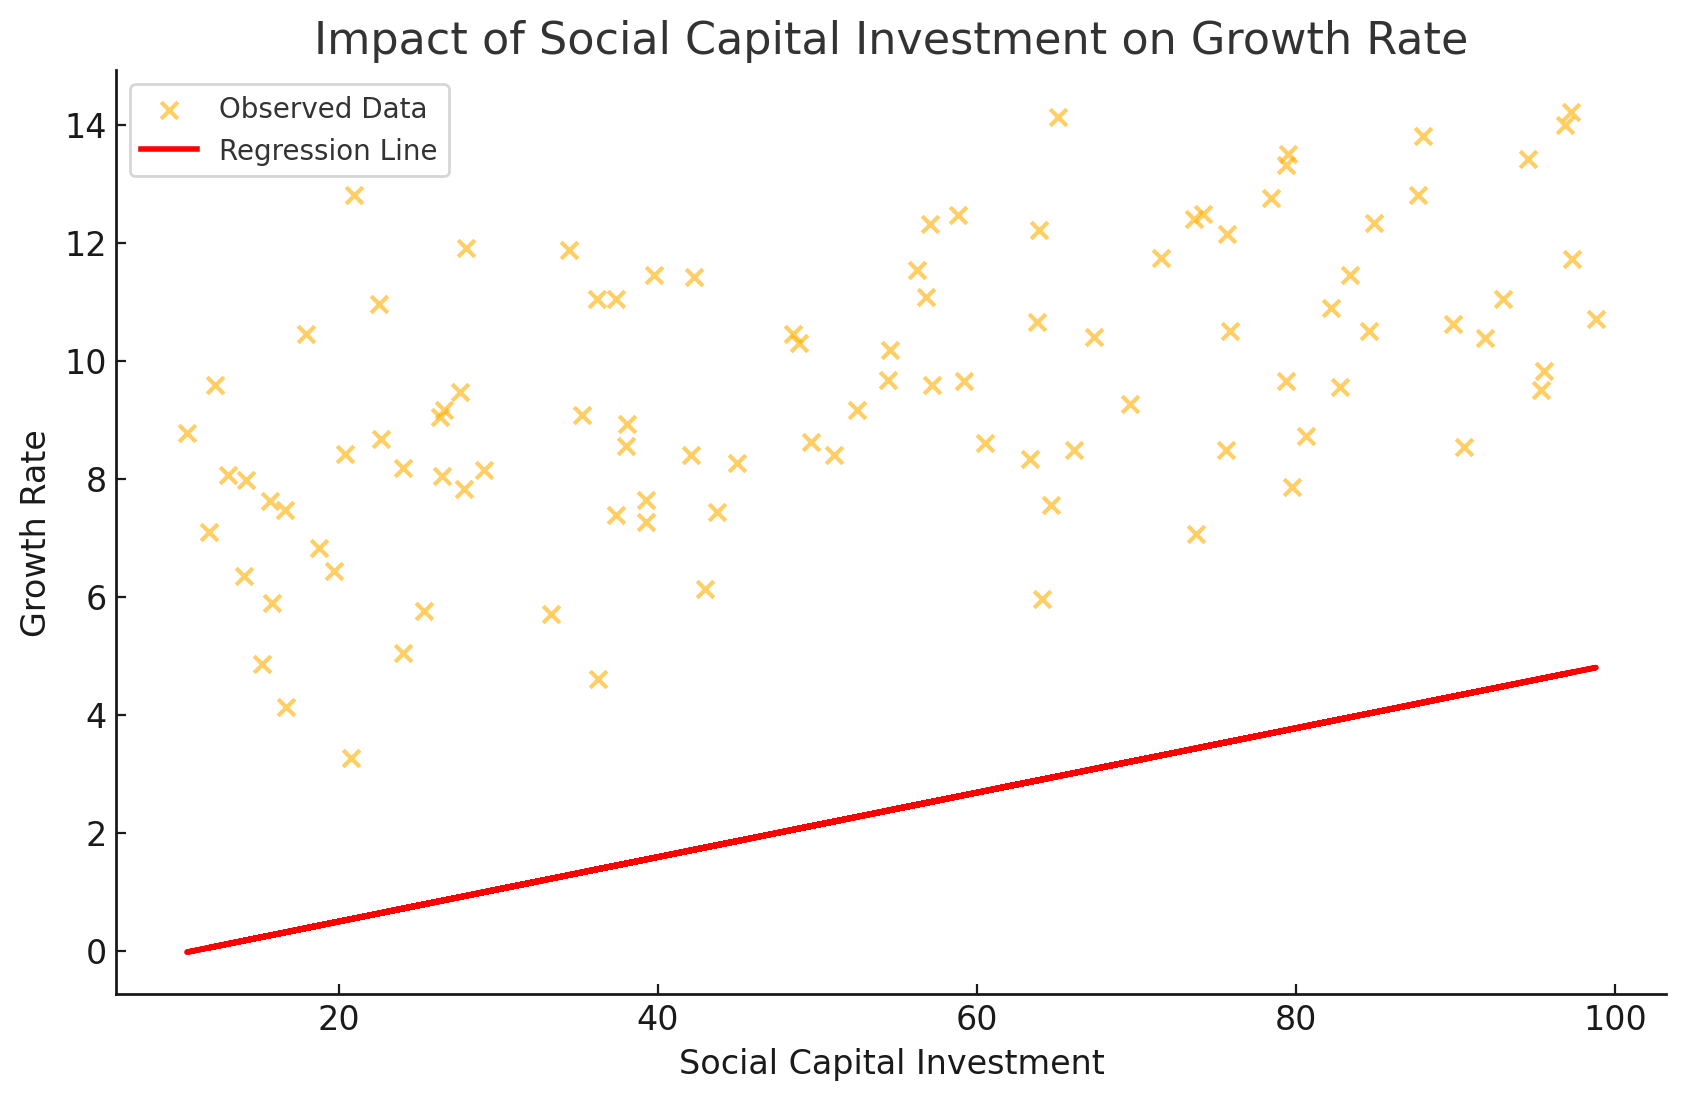
\includegraphics[width=0.4\textwidth]{figure/figure_sample.png}
	\caption{社会資本投資と経済成長率の回帰直線}
	\label{fig:regression_plot}
\end{figure}

本研究では,社会資本投資が地域経済に与える影響を分析し,特に経済成長率との関連性について検証を行った.その結果,社会資本投資が統計的に有意な正の効果を持つことが示され,経済成長における社会資本の重要性が確認された.つまり,社会資本投資は地域経済に多面的な影響を与える主要な政策手段であることが確認された.特に,TFPを通じた間接的な波及効果を考慮することで,社会資本投資の役割を包括的に理解することが可能となった.これにより,経済成長を支える要因としての社会資本の価値が理論的および実証的に再評価される意義を有する.

\section{おわりに}
分析結果から,社会資本投資の係数が民間資本や労働投入量と同程度の重要性を示したことから,社会資本が地域経済の基盤として生産性向上に貢献することが明らかになった.また,全要素生産性(TFP)を通じた間接的な波及効果を考慮することで,社会資本投資の長期的な成長促進効果を理論的および実証的に支持する結果が得られた.

政策的には,社会資本投資を戦略的に配分することで,地域間格差の是正や持続可能な経済成長を促進できる可能性が示唆された.また,社会資本投資の効果を最大化するためには,投資対象の種類や質,さらには人的資本や情報通信基盤との相乗効果を考慮する必要がある.


\setcitestyle{authoryear}
\bibliographystyle{backmatter/kucivil}
\bibliography{backmatter/references}

\end{document}